\documentclass[11pt,a4paper]{report}
\usepackage[utf8]{inputenc}\usepackage[T1]{fontenc}\usepackage[spanish]{babel}
\usepackage{geometry,graphicx,float,booktabs,longtable,tabularx,array,xcolor,listings,tcolorbox,fancyhdr,microtype,enumitem,hyperref,cleveref}
\geometry{margin=2.5cm}\definecolor{utecblue}{HTML}{092B49}\hypersetup{colorlinks=true,linkcolor=utecblue,urlcolor=utecblue,citecolor=utecblue}
\pagestyle{fancy}\fancyhf{}\lhead{ASTRA CLOUD}\rhead{Informe técnico}\cfoot{\thepage}
\newcommand{\Docente}{[Colchado Ruíz, Geraldo]}\newcommand{\IntegranteUno}{[Guerrero Cedron, Antonio Jorge]}\newcommand{\IntegranteDos}{[Huaman Huamani, Josue Yeremi]}\newcommand{\IntegranteTres}{[Timana Carmona, Jose Manuel]}\newcommand{\IntegranteCuatro}{[Villalobos Jiménez, José Luis]}\newcommand{\IntegranteCinco}{[Rosales Esteban, Antony Yonel]}
\lstset{basicstyle=\ttfamily\footnotesize,breaklines=true,frame=single,captionpos=b}
\begin{document}
\begin{titlepage}\centering\vspace*{1cm}{\Large UNIVERSIDAD DE INGENIERÍA Y TECNOLOGÍA\\UTEC\par}\vspace{1cm}\fbox{\parbox[c][2cm][c]{.5\textwidth}{\centering ESPACIO PARA LOGO UTEC}}\vfill{\large Curso: CLOUD COMPUTING\par}\vspace{.6cm}{\color{utecblue}\bfseries\LARGE DISEÑO E IMPLEMENTACIÓN DE UNA ARQUITECTURA CLOUD\\BASADA EN MICROSERVICIOS PARA ASTRA CLOUD\par}\vspace{.6cm}{\Large Informe Técnico del Proyecto\par}\vfill\begin{tabular}{rl}Docente:&\Docente\\Integrantes:&\IntegranteUno\\&\IntegranteDos\\&\IntegranteTres\\&\IntegranteCuatro\\&\IntegranteCinco\end{tabular}\vfill Lima -- Perú\\2026\end{titlepage}
\tableofcontents\listoffigures\listoftables\clearpage
\chapter{Introducción} ASTRA CLOUD es una plataforma cinematográfica distribuida. Este informe es una auditoría estática de siete repositorios públicos clonados el 22 de septiembre de 2026 y del directorio de trabajo, inicialmente vacío. Las afirmaciones implementadas se trazan a rutas de los repositorios bajo \texttt{sources/}; la infraestructura solicitada no se encontró y se reporta como no verificable.
\chapter{Objetivos}\section{Objetivo general}Documentar técnicamente la implementación verificable de ASTRA CLOUD.\section{Objetivos específicos}\begin{itemize}\item Reconstruir servicios, persistencia y comunicaciones.\item Distinguir código, configuración y recomendaciones.\item Identificar límites y riesgos observables.\end{itemize}
\chapter{Descripción del proyecto}\section{Problema y solución}El código implementa catálogo, identidad, comunidades, interacciones, sesiones de visualización y consultas analíticas. No se encontró frontend; su implementación no se pudo verificar.\section{Alcance}El alcance comprobado es API REST, WebSocket en sesiones, persistencia poliglota y extracción hacia S3.\section{Requerimientos}Las rutas verificadas habilitan registro/inicio de sesión, películas, clubes, salas, reseñas, ``likes'', listas y métricas. Los requisitos no funcionales verificables incluyen contenedores y endpoints de salud; no se encontró evidencia de SLA.
\chapter{Arquitectura general}\section{Visión general}Como se observa en la Figura~\ref{fig:arquitectura_general}, el diseño suministrado se contrasta con la plantilla CloudFormation. Esta define seis HTTP API Gateway, un VPC Link, ALB interno y seis servicios en dos EC2 de producción.\begin{figure}[H]\centering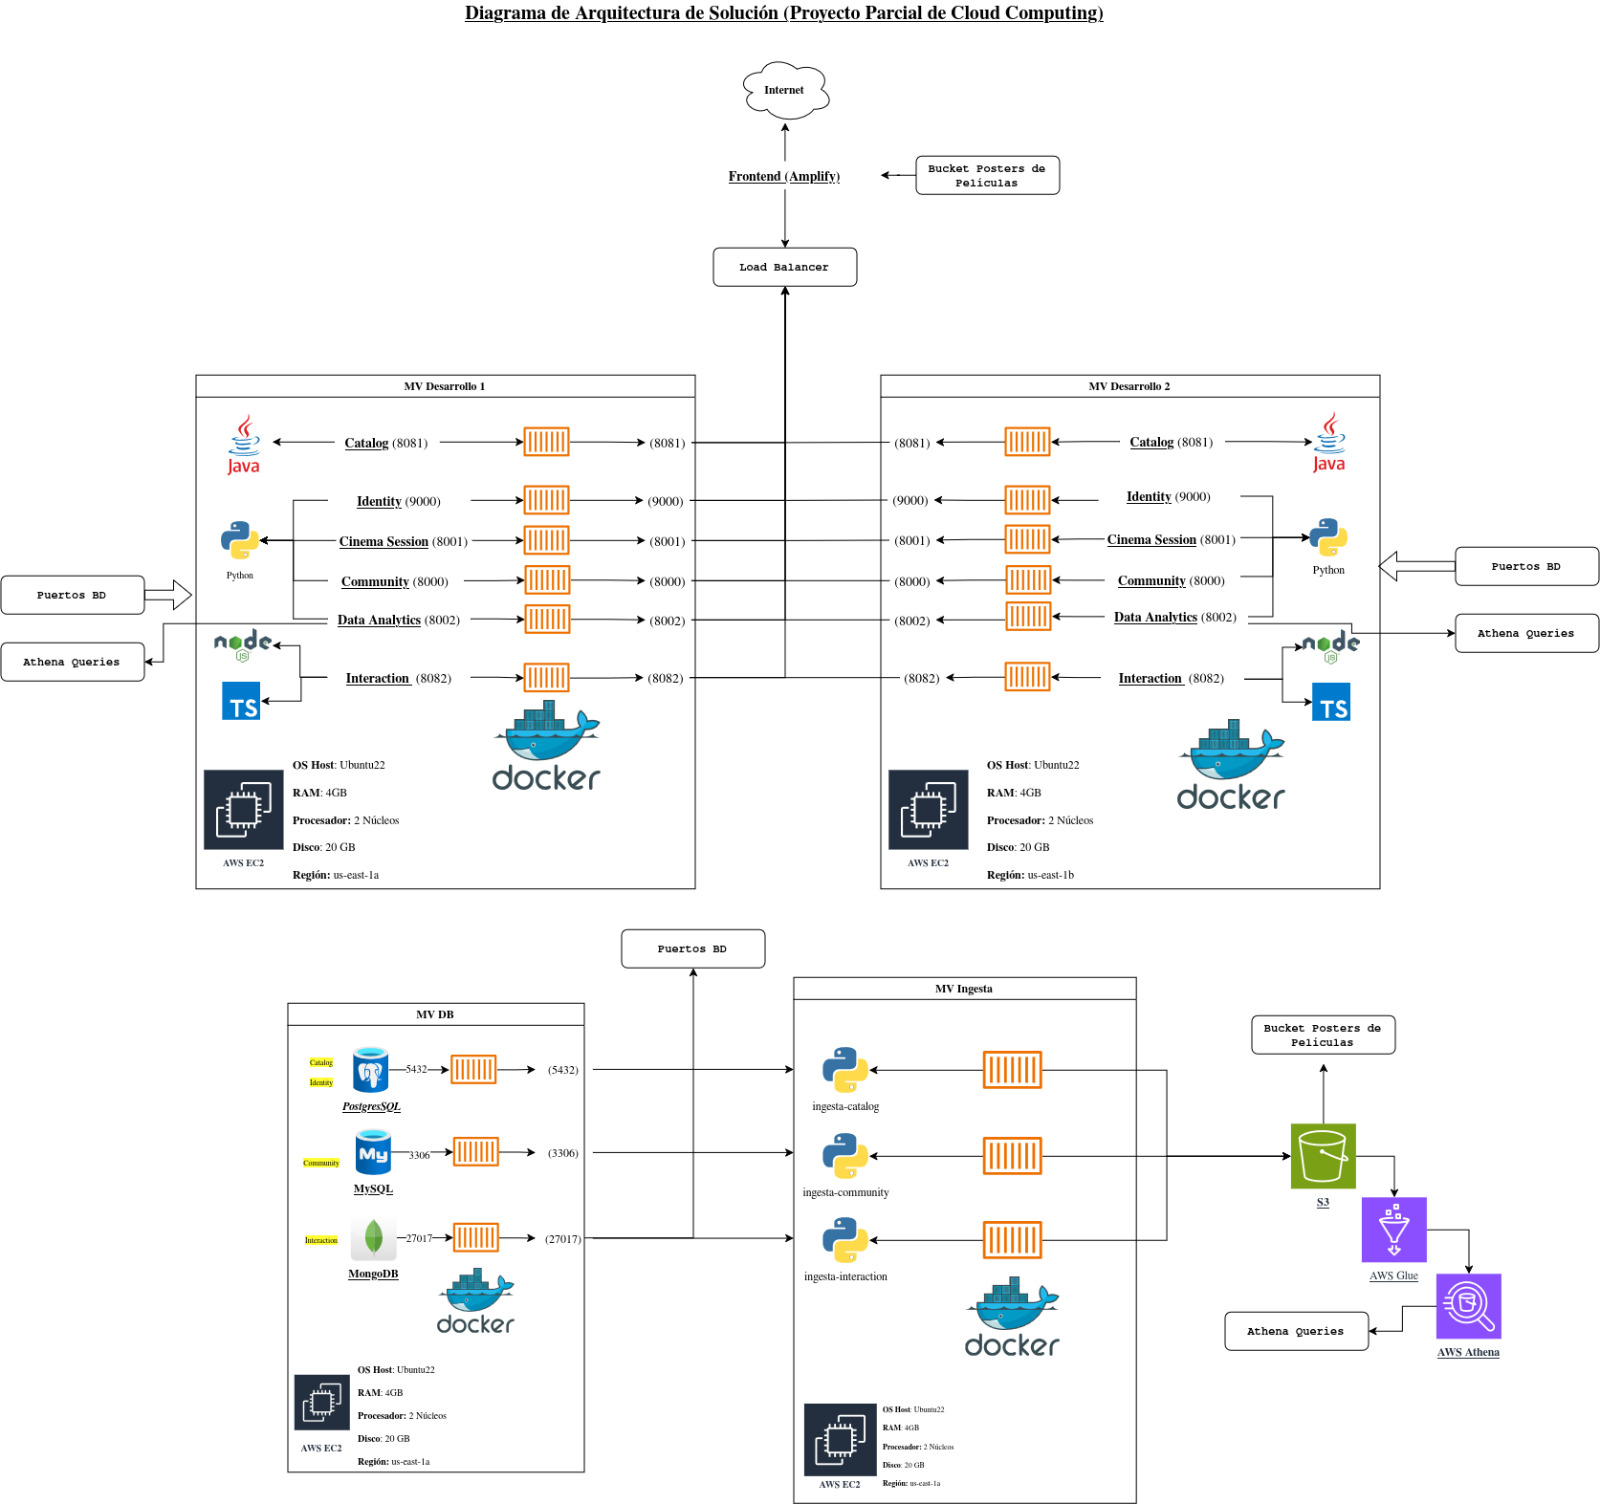
\includegraphics[width=\textwidth]{figures/arquitectura-general.jpeg}\caption{Arquitectura general de Astra Cloud}\label{fig:arquitectura_general}\end{figure}\section{Flujo}La ruta definida es cliente $\rightarrow$ API Gateway $\rightarrow$ VPC Link $\rightarrow$ ALB interno $\rightarrow$ listener por puerto $\rightarrow$ target group $\rightarrow$ EC2 $\rightarrow$ contenedor. El ALB no es entrada pública directa: su \texttt{Scheme} es \texttt{internal}. La plantilla define recursos; no prueba su despliegue actual.
\chapter{Arquitectura de microservicios}
\section{Catálogo de APIs verificables}Las rutas siguientes provienen de controladores y routers; los prefijos FastAPI se obtienen de sus routers.
\begin{longtable}{p{.13\textwidth}p{.12\textwidth}p{.37\textwidth}p{.3\textwidth}}\caption{Catálogo resumido de APIs}\toprule Servicio&Método&Ruta&Propósito\\\midrule\endfirsthead\toprule Servicio&Método&Ruta&Propósito\\\midrule\endhead Catalog&GET&/api/catalog/home, /search&Home y búsqueda.\\Catalog&GET/POST&/api/catalog/movies, /\{publicId\}, /session-info&Catálogo y detalle para sesión.\\Identity&POST&/register, /login&Alta y autenticación JWT.\\Community&CRUD&/api/v1/users, /clubs, /watch-rooms&Perfiles, clubes y salas.\\Interaction&GET/POST/PUT/DELETE&/api/v1/reviews, /movies/:id/like, /users/:id/watchlist&Interacciones documentales.\\Cinema&POST/PATCH/GET&/api/v1/sessions, /:id/playback, /:id/state, /:id/chat&Sesión activa.\\Analytics&GET&/top-watched, /kpis, /movies/best-rated&Consultas Athena.\\\bottomrule\end{longtable}
\section{Catalog Service}
Catalog concentra el catálogo cinematográfico. Su código Java Spring Boot se organiza en controladores \texttt{CatalogController}, \texttt{MovieController} y \texttt{HealthController}, servicios, repositorios JPA y entidades. Una petición sigue Controller $\rightarrow$ Service $\rightarrow$ Repository $\rightarrow$ PostgreSQL; los DTO separan la respuesta pública de entidades. \texttt{Movie} es la entidad principal y se relaciona con géneros, artistas, fuentes de video y subtítulos; \texttt{MovieVideoSource} y \texttt{MovieSubtitle} pertenecen al detalle reproducible. \texttt{MovieRepository} usa \texttt{EntityGraph} para cargar relaciones requeridas. La configuración JDBC apunta a PostgreSQL y el contenedor expone 8081. En IaC, Catalog recibe API Gateway $\rightarrow$ VPC Link $\rightarrow$ ALB interno 8081 $\rightarrow$ TGCatalog $\rightarrow$ ambas EC2 Prod. Un GET de película atraviesa ese recorrido, busca por UUID público mediante controlador/servicio/repositorio y devuelve JSON. No se verificó un middleware de autorización propio en los controladores auditados.
\section{Identity Service}
Identity es la autoridad de cuentas y tokens. FastAPI registra \texttt{/register} y \texttt{/login}; \texttt{models.py} define \texttt{users} con UUID, email único, nombre, hash y rol. En registro, Pydantic valida el cuerpo, el servicio consulta la unicidad, aplica hash de contraseña y persiste SQLAlchemy. En login, consulta usuario, verifica hash y \texttt{core/security.py} emite JWT HS256 con \texttt{sub}, \texttt{exp} e \texttt{iss=identity-service}. El secreto y la expiración proceden de configuración, no se reproducen valores. El contenedor escucha 9000; IaC define IdentityAPI, listener 9000 y TGIdentity con las dos EC2.\section{Community Service}
Community persiste la capa social: \texttt{users} locales asociados al \texttt{sub} de Identity, \texttt{clubs}, \texttt{memberships}, \texttt{watch\_rooms} y \texttt{watch\_participants}. Un club tiene propietario, visibilidad y miembros; Membership vincula usuario-club con rol OWNER/ADMIN/MEMBER; WatchRoom identifica película, anfitrión y club opcional; Participant registra nickname y rol HOST/VIEWER. \texttt{deps.py} valida Bearer JWT, exige issuer y puede crear el perfil local en el primer acceso autenticado. Por ello Community no almacena contraseñas ni emite tokens. Rutas verificables incluyen GET/PUT usuarios, CRUD clubes, altas/listas de membresía y POST/GET/join de watch rooms. Usa FastAPI, SQLAlchemy y MySQL en 8000.
\section{Interaction Service}
Interaction implementa escritura social de alta variabilidad con Node.js, Express, Mongoose y MongoDB. \texttt{auth.js} extrae Bearer, verifica JWT con algoritmo configurado y coloca identidad para rutas protegidas. Review contiene \texttt{movie\_id}, \texttt{user\_id}, score 0--10, comentario, fecha y snapshots movie/user; Like contiene identificadores, fecha y snapshots. Watchlist e historial usan el mismo patrón de contexto embebido. Los índices por movie, user y el compuesto único movie/user en Review y Like impiden duplicados. El recorrido de un like es HTTP $\rightarrow$ authenticate $\rightarrow$ movie route $\rightarrow$ controlador $\rightarrow$ modelo Mongoose $\rightarrow$ MongoDB; reseña, lista e historial siguen la misma separación. Las rutas incluyen crear/listar/editar/borrar reseñas, like/unlike, métricas, watchlist e historial; los endpoints de ingesta están protegidos por clave específica.
\section{Cinema Session Service}
La rama auditada es \texttt{feature/http-polling-chat}. Community persiste una watch room; Cinema administra el estado activo transitorio de una sesión sincronizada. \texttt{session\_service.py} crea sesiones, consulta película en Catalog y consulta room en Community; mantiene datos en memoria. Las rutas permiten crear/listar/obtener/borrar sesiones, añadir/quitar/listar participantes, PATCH playback, GET state y POST chat. El cliente puede obtener estado por HTTP polling mediante GET state; además \texttt{ws.py} define WebSocket para eventos y chat. Ambos mecanismos coexisten: no se describe como exclusivamente polling. Cinema consulta Interaction para estadísticas/likes con timeout de dos segundos en las llamadas visibles. Un PATCH playback actualiza el estado local; otro cliente puede recibir evento WebSocket o consultar GET state. Con dos EC2 detrás de ALB, solicitudes consecutivas pueden caer en réplicas distintas: si no comparten memoria, una sesión creada en Prod1 puede no existir en Prod2.\section{Data Analytics Service}
Analytics no accede al OLTP en sus rutas: FastAPI delega a \texttt{app/athena/client.py}. Este crea cliente boto3, envía \texttt{StartQueryExecution}, sondea el estado y devuelve filas cuando alcanza SUCCEEDED; FAILED y CANCELLED se tratan como terminales. \texttt{ATHENA\_OUTPUT\_BUCKET} configura resultados. Rutas verificables cubren top watched, actor/género, mejor calificación, likes, actividad social, KPIs, embudo, retención y salud de clubs. El contenedor expone 8002 y la plantilla define AnalyticsAPI/TGAnalytics.
\chapter{Persistencia políglota}
\section{PostgreSQL} Catalog configura JDBC PostgreSQL e Identity define \texttt{users}. La Figura~\ref{fig:er_postgresql}, trazable en \texttt{evidence/er-postgresql-sources.md}, resume \texttt{users} (PK UUID, email único/indexado) y las entidades Catalog \texttt{movie}, \texttt{genre}, \texttt{artist}, \texttt{movie\_video\_source} y \texttt{movie\_subtitle}. No se afirma una FK interservicio no presente en código.
\begin{figure}[H]
    \centering
    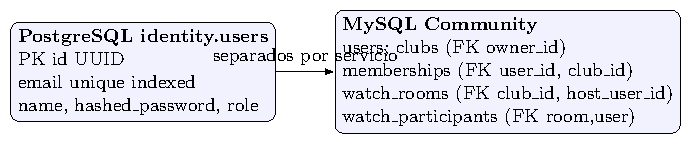
\includegraphics[width=0.95\textwidth]{figures/er-postgresql.pdf}
    \caption{Modelo entidad--relación de la persistencia PostgreSQL de Astra Cloud}
    \label{fig:er_postgresql}
\end{figure}
La PK UUID identifica cuentas; las entidades Catalog representan el dominio cinematográfico en persistencia relacional.
\section{MySQL} Community define \texttt{users}, \texttt{clubs}, \texttt{memberships}, \texttt{watch\_rooms} y \texttt{watch\_participants}; las FK verificadas constan en \texttt{evidence/er-mysql-sources.md}. La Figura~\ref{fig:er_mysql} representa las relaciones verificables.
\begin{figure}[H]
    \centering
    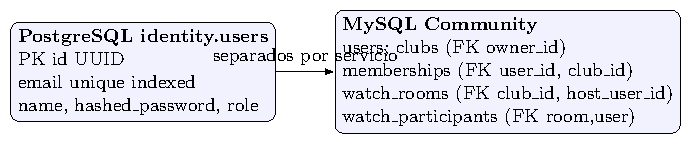
\includegraphics[width=0.95\textwidth]{figures/er-mysql.pdf}
    \caption{Modelo entidad--relación de la persistencia MySQL de Astra Cloud}
    \label{fig:er_mysql}
\end{figure}
\texttt{clubs.owner\_id} y \texttt{watch\_rooms.host\_user\_id} referencian usuarios; \texttt{memberships} materializa la relación N:M usuario--club.
\section{MongoDB} Interaction usa \texttt{Review}, \texttt{Like}, \texttt{Watchlist} y \texttt{WatchHistory}. La Figura~\ref{fig:modelo_mongodb} representa snapshots embebidos; \texttt{movie\_id} y \texttt{user\_id} son números de aplicación, no \texttt{ObjectId}, según \texttt{evidence/mongodb-model-sources.md}.
\begin{figure}[H]
    \centering
    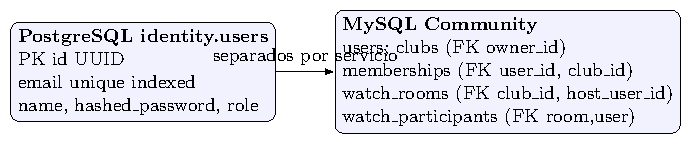
\includegraphics[width=0.95\textwidth]{figures/modelo-mongodb.pdf}
    \caption{Modelo documental MongoDB del Interaction Service}
    \label{fig:modelo_mongodb}
\end{figure}
Los índices compuestos únicos de Review y Like evitan repetir interacción por película y usuario.\begin{lstlisting}[caption={Documento Review derivado de review.js},label={lst:review-json}]
{"movie_id":42,"user_id":7,"score":8,"comment":"","date":"<Date>",
 "movie":{"id":42,"title":"...","poster_url":"..."},
 "user":{"id":7,"username":"...","display_name":"...","avatar_url":"..."}}
\end{lstlisting}
\begin{table}[H]\centering\caption{Bases de datos}\begin{tabularx}{\textwidth}{llllX}\toprule Motor&Servicio&Puerto&Modelo&Justificación\\\midrule PostgreSQL&Catalog, Identity&5432 config.&Relacional&JDBC/SQLAlchemy.\\MySQL&Community&3306 config.&Relacional&Configuración MySQL.\\MongoDB&Interaction&No verificado&Documental&Mongoose.\\\bottomrule\end{tabularx}\end{table}
\chapter{Comunicación entre microservicios}\begin{table}[H]\centering\caption{Comunicación verificable}\begin{tabularx}{\textwidth}{lllX}\toprule Origen&Destino&Protocolo&Propósito\\\midrule Cinema&Catalog&HTTP GET&Valida/obtiene película.\\Cinema&Community&HTTP GET&Consulta watch-room.\\Cinema&Interaction&HTTP GET&Estadísticas y likes.\\Analytics&Athena&SDK boto3&Ejecuta SQL analítico.\\\bottomrule\end{tabularx}\end{table}\texttt{session\_service.py} usa URLs configurables y timeouts de dos segundos para algunas consultas. El estado de sesión en memoria hace que múltiples réplicas no compartan estado; es una inferencia directa de la ausencia de persistencia en el servicio.
\chapter{Contenedorización}\section{Compose contrastado}Los Compose proporcionados definen Catalog 8081, Community 8000, Interaction 8082, Analytics 8002, Identity 9000 y Cinema 8001; la plantilla usa imágenes \texttt{villabos/*:v2}, Analytics v3 y reinicio \texttt{unless-stopped}. DB Compose usa PostgreSQL 16, MySQL 8.4.6 y MongoDB 7 con volúmenes. Ingesta define tres contenedores con prefijos S3 \texttt{resultados/catalogo}, \texttt{comunity} e \texttt{iteraction}. Los Compose locales con credenciales en texto plano son un riesgo; se omiten sus valores.
\chapter{Infraestructura AWS}\section{CloudFormation definido}La plantilla define VPC \texttt{10.0.0.0/16}, subredes públicas \texttt{10.0.1.0/24} y \texttt{10.0.2.0/24} en las dos primeras AZ, IGW, ruta \texttt{0.0.0.0/0}, DNS habilitado y zona privada Route53 \texttt{proycloud.local}. El registro \texttt{db.proycloud.local} apunta a la IP privada de DB. Define cuatro EC2 \texttt{t3.medium}, EBS gp3 de 20 GiB: DB e Ingesta en subnet 1; Prod 1 en subnet 1 y Prod 2 en subnet 2. User Data instala Docker y ejecuta Compose.\section{Exposición}Se definen seis HTTP APIs, VPC Link, integraciones \texttt{HTTP\_PROXY} y listeners/target groups en 8000,8001,8002,8081,8082,9000. Cada grupo registra ambas EC2 Prod y consulta \texttt{/health} cada 30 s. S3 de posters tiene cifrado SSE-S3 AES256 y lectura pública de objetos.\begin{table}[H]\centering\caption{API Gateway y destinos definidos}\begin{tabularx}{\textwidth}{l l l X}\toprule Servicio&API&Puerto/TG&Instancias\\\midrule Identity&IdentityAPI&9000/TGIdentity&Prod1, Prod2\\Catalog&CatalogAPI&8081/TGCatalog&Prod1, Prod2\\Community&CommunityAPI&8000/TGCommunity&Prod1, Prod2\\Interaction&InteractionAPI&8082/TGInteraction&Prod1, Prod2\\Analytics&AnalyticsAPI&8002/TGAnalytics&Prod1, Prod2\\Cinema&CinemaAPI&8001/TGCinema&Prod1, Prod2\\\bottomrule\end{tabularx}\end{table}
\chapter{Alta disponibilidad y balanceo}CloudFormation define dos réplicas de producción en AZ distintas y un ALB interno multi-subnet. Los seis target groups apuntan a ambas, con health check \texttt{/health} cada 30 s; una réplica no saludable dejaría de recibir tráfico del grupo. No se define Auto Scaling Group. DB e Ingesta son instancias únicas y constituyen SPOF. Cinema mantiene estado en memoria: aunque el ALB balancee, las réplicas no comparten sesiones.
\chapter{Pipeline de datos}\texttt{ingesta-catalogo/ingest.py} extrae PostgreSQL; \texttt{ingesta-comunity/ingest.py}, MySQL; y \texttt{ingesta-iteraction/ingest.py}, MongoDB. Cada uno usa boto3 para cargar a S3. No se verificó frecuencia programada ni Glue desde IaC.\begin{table}[H]\centering\caption{Pipeline analítico}\begin{tabularx}{\textwidth}{lXX}\toprule Etapa&Tecnología&Salida\\\midrule Extracción&psycopg2/pymysql/pymongo&Datos serializados.\\Carga&boto3 S3&Objeto en bucket configurable.\\Consulta&boto3 Athena&Resultado de consulta.\\\bottomrule\end{tabularx}\end{table}
\chapter{Analítica serverless}\texttt{app/athena/client.py} inicia ejecución Athena y realiza polling hasta \texttt{SUCCEEDED}, \texttt{FAILED} o \texttt{CANCELLED}. La separación OLTP/analítica se implementa parcialmente por las extracciones a S3 y consultas Athena; Glue Data Catalog no pudo verificarse. El análisis evita que rutas Analytics consulten directamente los motores transaccionales.
\chapter{Seguridad}\section{JWT}Identity emite JWT HS256; Community, Interaction y Cinema los validan con secreto compartido.\section{Riesgos}Se encontraron valores por defecto \texttt{change-me-in-production} en configuración de Cinema e Interaction. No se reproducen secretos: cualquier valor real debe tratarse como \texttt{[REDACTED]}. Se recomienda migrar secretos a Secrets Manager o SSM, como propuesta. Security Groups, CORS, TLS y cifrado no se pudieron verificar sin infraestructura.\begin{table}[H]\centering\caption{Variables de entorno importantes}\begin{tabularx}{\textwidth}{l l X}\toprule Variable&Componente&Propósito\\\midrule JWT\_SECRET / JWT\_SECRET\_KEY&Identity/Community/Cinema/Interaction&Firma o validación JWT.\\DATABASE\_URL&Identity&Conexión SQLAlchemy.\\ATHENA\_OUTPUT\_BUCKET&Analytics&Resultados Athena.\\PG\_*/MYSQL\_*/MONGO\_URI&Ingestas&Origen OLTP.\\\bottomrule\end{tabularx}\end{table}
\chapter{Infraestructura como código}No se encontró plantilla CloudFormation. En consecuencia, no se puede evaluar recursos automatizados, User Data ni reproducibilidad de infraestructura. Esta conclusión contradice la premisa de que \texttt{proycloud-infrastructure.yaml} estaba disponible.
\chapter{Flujos funcionales}\section{Autenticación}\begin{enumerate}\item Cliente envía credenciales a \texttt{/register} o \texttt{/login} de Identity.\item \texttt{core/security.py} genera JWT.\item Community, Interaction y Cinema validan el Bearer con secreto compartido.\end{enumerate}\section{Catálogo}\begin{enumerate}\item Cliente consulta controlador Catalog.\item Spring procesa y accede a PostgreSQL configurado.\end{enumerate}\section{Interacción}\begin{enumerate}\item Middleware Interaction verifica JWT.\item Ruta persiste documento Mongoose y responde JSON.\end{enumerate}\section{Comunidad y sesión}\begin{enumerate}\item Community crea sala.\item Cinema consulta sala y película por HTTP; mantiene sesión local.\item WebSocket distribuye eventos a participantes conectados.\end{enumerate}\section{Consulta analítica}\begin{enumerate}\item Ingesta extrae OLTP y sube S3.\item Analytics envía SQL a Athena y sondea finalización.\end{enumerate}
\chapter{Pruebas y validación}Se hallaron pruebas en \texttt{community/tests}, \texttt{interaction/tests} y \texttt{cinema/tests}. No se ejecutaron porque el informe no contó con servicios, variables ni bases de datos configuradas.\begin{figure}[H]\centering\fbox{\parbox[c][6cm][c]{.9\textwidth}{\centering\textbf{EVIDENCIA PENDIENTE}\\Capturas de health checks, EC2, Target Groups, API Gateway, S3, Athena, frontend y contenedores.}}\caption{Evidencia operativa pendiente}\label{fig:evidencia_pendiente}\end{figure}
\chapter{Análisis de costos}El gasto real no puede calcularse sin región, uso y configuración. Si se despliegan los recursos descritos en el enunciado, deben presupuestarse EC2, EBS, ALB, API Gateway, S3, Athena, Glue y transferencia. Su existencia no quedó verificada por artefactos.
\chapter{Limitaciones actuales}\begin{itemize}\item El estado en memoria de Cinema dificulta escalamiento horizontal consistente.\item JWT HS256 exige distribución segura del secreto entre servicios.\item No hay evidencia de infraestructura, backups, observabilidad, TLS ni autoscaling.\item No se verificó programación de ingestas ni Glue.\end{itemize}\section{Consistencia entre diseño e implementación}\begin{table}[H]\centering\caption{Consistencia entre diseño e implementación}\begin{tabularx}{\textwidth}{lXXX}\toprule Elemento&Diagrama&Código/infraestructura&Estado\\\midrule Diagrama general&Archivo no disponible&No contrastable&NO VERIFICADO\\CloudFormation&No disponible&No encontrado&NO VERIFICADO\\S3/Athena&No contrastable&boto3 en ingesta/Analytics&VERIFICADO\\Cinema HTTP polling&No contrastable&No se encontró frecuencia; WebSocket presente&PARCIALMENTE VERIFICADO\\\bottomrule\end{tabularx}\end{table}
\chapter{Mejoras futuras}Estas propuestas no están implementadas: almacenar el estado de sesión en Redis para réplicas; usar Secrets Manager; incorporar CloudWatch, backups y alertas; usar Auto Scaling Groups y balanceador; sustituir polling por WebSocket cuando el cliente no lo use; y definir CI/CD con escaneo de imágenes.
\chapter{Conclusiones}La evidencia sostiene una separación por dominios y persistencia PostgreSQL, MySQL y MongoDB, además de ingesta a S3 y consultas Athena. Cinema presenta una dependencia de estado local que condiciona su escalamiento. La arquitectura AWS declarada por el enunciado no puede certificarse sin su plantilla; el informe preserva esta distinción para no convertir diseño supuesto en implementación.

\nocite{*}\bibliographystyle{plain}\bibliography{references}\end{document}
